\documentclass[11pt]{article}
\usepackage[a4paper]{geometry}
\usepackage{kotex}
\usepackage{hyperref}
\usepackage{subcaption}
\usepackage{caption}
\usepackage{graphicx}
\usepackage{float}
\hypersetup{
    colorlinks,
    citecolor=black,
    filecolor=black,
    linkcolor=black,
    urlcolor=black
}
\usepackage[
    type={CC},
    modifier={by-nc-sa},
    version={3.0},
]{doclicense}

\title{Marina Bay sands tutorial}
\author{채희진}
\date{\today}

\renewcommand{\abstractname}{초록}

\begin{document}
    

\maketitle
\thispagestyle{empty}
\clearpage

\doclicenseThis
\thispagestyle{empty}
\clearpage

\tableofcontents
\thispagestyle{empty}
\clearpage

\pagenumbering{arabic}

\begin{abstract}
   \href{https://www.safdiearchitects.com/projects/marina-bay-sands-integrated-resort}{Marina Bay Sands(MBS)}는 Safdie라는 콧수염난 아저씨가 차린 회사에서 한 프로젝트로, Autodesk University에 MBS 및 Changi 공항 프로젝트가 올라온 바 있습니다. 
   본 노트에서는 Dynamo를 이용해 구성되어 있던 예제를 이해해서 Grasshopper로 만들고, 이 과정에서 필요한 실무적인 지식을 소개합니다. 
\end{abstract}

\section{레이어 관리}
그래스호퍼를 위주로 설명하지만, 실무 상황을 가정하고 몇가지 다른이야기도 섞어서 소개하도록 하겠습니다. 프로젝트를 하면서 가장 중요한 것 중 하나는 레이어 관리입니다.
 가장 좋은 상황은 모든 팀이 정해놓은 따라 레이어를 쓴다면 고생할 일이 없지만, 대부분 상황에서는 레이어 표준이라는 개념이 희박합니다. 또한 건축 특성상 프로젝트별 차이가 있기 때문에
 각 상황에서 문재렬 해결하기 위한 가장 유용한 판단을 내리는 것이 중요합니다.

 레이어 이름을 정할때 Product breakdown structure(PBS)에 따라 하는게 제일 좋습니다. 즉, 건물을 하나의 제품으로 보고, 프로젝트 안에 건물과 대지, 건물 안에 층, 층 안에 벽 등등으로 좁혀 나가는 방식입니다.
 Ghery techonologies(GT)에서도 여기에 기반해 레이어를 만들고 관리를 하고 있는 것으로 알고있고, 특이한점은 꼭 영어 알파벳 3자리를 고집한다는 것입니다. 

 예를 들어, Marina bay sands라면 MBS로 가장 상위 레이어를 정하고, 그아래 DRV(Driver, 핵심 지오메트리), FAC(Facade, 외피), SIT(Site, 대지) 등으로 구분하는 방식입니다(Figure \ref{fig:ghery_example}). 해당 구조를 통해 레이얼르 구성하면 
 MBS-DRV 이런식으로 구성이 가능 합니다. 이렇게 3글자를 기준으로 하면 레이어 이름이 과도하게 늘어나는 것을 방지할 수 있습니다. 하지만 때로는 지나치게 줄여서 어떤의미인지 어려울 때도 있습니다.
 제 개인적인 의견은 3글자인지 4글자인지가 중요한게 아니고, PBS를 적용했다는 것이고 프로그래밍 측면에서 보면 중간에 대시(-)를 일관적으로 넣는 일이 더 중요하다고 생각합니다.
 왜냐하면 프로젝트를 할때 레이어 이름을 이용해서 작업을 하는 경우도 있기 때문입니다.
 \begin{figure}[H]
    \centering
    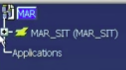
\includegraphics[width=.3\textwidth]{./img/ghery_example}
    \caption[Caption for LOF]{GT에서 사용하는 레이어 관리 방식\footnotemark}
    \label{fig:ghery_example}
 \end{figure}

\footnotetext{\href{https://youtu.be/hr4Vk5lGucU?t=129}{https://youtu.be/hr4Vk5lGucU?t=129}}
다시 돌아와 레이어를 정리해보도록 하겠습니다. 레이어를 정리할때 핵심은 그래스호퍼의 입력값으로 들어갈 값들을 잘 정리하는 것입니다. 본 프로젝트에서는 가장 상위 구조를 MBS로 정했습니다. 그리고 눈으로 확인용으로 쓰는 주변 Geoemtry들은 \textit{MBS-Context}에 포함시켰고,
Grasshopper의 입력값으로 사용될 예정인 값들은 \textit{MBS-Driver}아래에 각각 분리해서 정리했습니다(Figure \ref{fig:layer_before_after}).

\begin{figure}[H]
    \centering
    \begin{subfigure}{.45\textwidth}
        \centering
        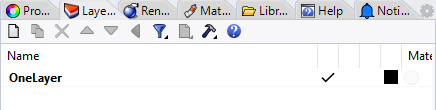
\includegraphics[width=.9\textwidth]{./img/mbs_layer_before}
        \caption{레이어 정리 전}
        \label{fig:mbs_layer_before}
    \end{subfigure}
    \begin{subfigure}{.45\textwidth}
        \centering
        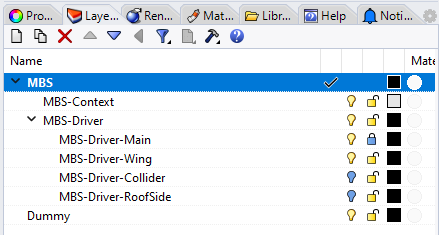
\includegraphics[width=.9\textwidth]{./img/mbs_layer_after}
        \caption{레이어 정리 후}
        \label{fig:mbs_layer_after}
    \end{subfigure}
    \caption{레이어 정리 전후 비교}
    \label{fig:layer_before_after}
\end{figure}

이번 강의에서 다룰 주요 지오메트리는 하단부의 반원 모양입니다. 해당 지오메트리를 \textit{MBS-Driver-main} 아래에 넣어놓았습니다(Figure \ref{fig:mbs_layer_main}).
 다른 지오메트리들도 일단은 구분해서 넣어놨고, 추후에 몇몇 지오메트리에 대한 패널링도 진행할 예정입니다.

\begin{figure}[H]
    \includegraphics*[width=\textwidth]{./img/mbs_layer_main.png}
    \caption{패널링을 수행할 지오메트리}
    \label{fig:mbs_layer_main}
\end{figure}
\pagebreak
% section 
\section{지오메트리 상태 확인}
그래스호퍼, 다이나모 등을 이용할 때 가장 중요한 일은 지오메트리의 상태를 확인하는 것입니다. 왜냐하면 지오메트리의 성격에 따라 실행해야 하는 커멘드가 다르기 때문입니다. 이와 밀접한 특성은 위상학(topology) 입니다.
이번 스크립트에서는 아주 간단하게 untrim이라는 커맨드만 넣어 지오메트리를 확인했는데(Figure \ref{fig:mbs_01_check}), 이와 관련된 이야기를 잠시 해보도록 하겠습니다.

\begin{figure}[H]
    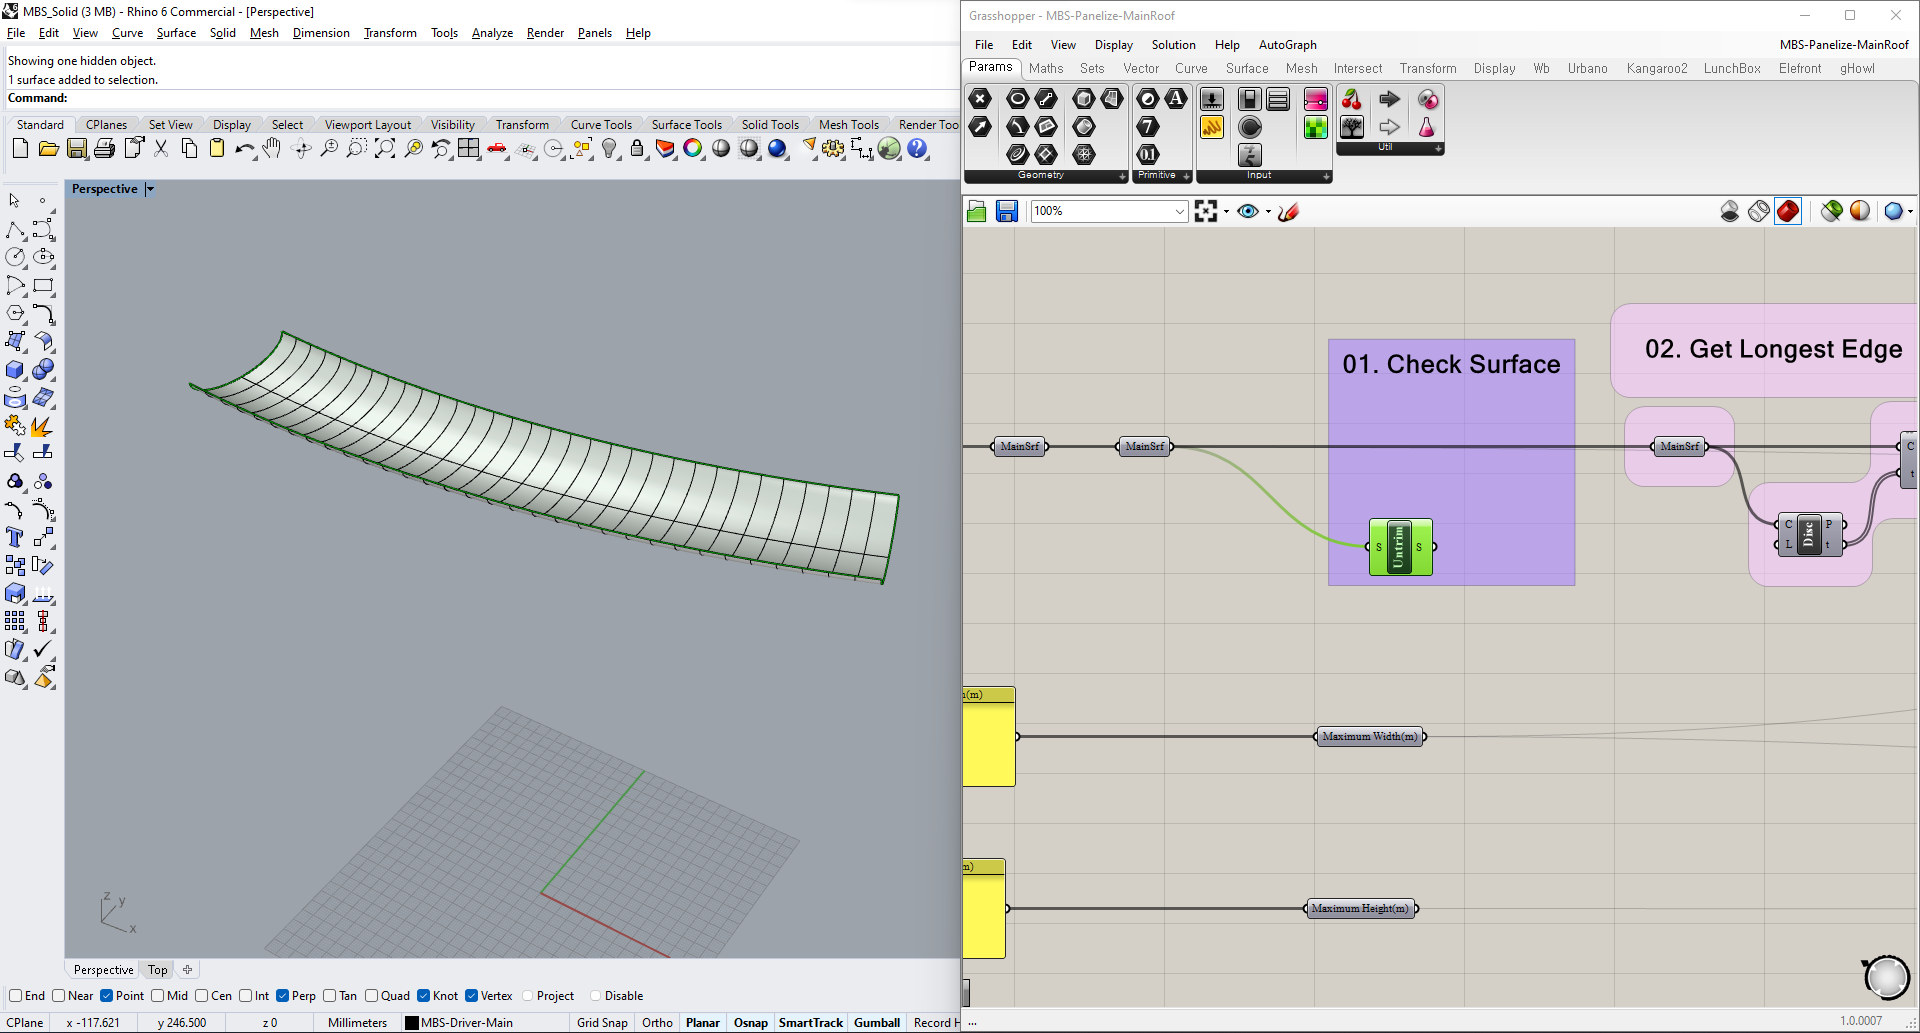
\includegraphics[width=\textwidth]{./img/mbs_01_check.png}
    \caption{Untrim을 이용한 지오메트리 상태 확인}
    \label{fig:mbs_01_check}
\end{figure}

\subsection{위상학(Topology)}
컴퓨터 그래픽이나 지오메트리에 대해서 이야기하시는 분들은 위상학을 많이 이야기 하십니다. 그중 특히 자주 나오는 예시는 도넛과 머그컵입니다(Figure \ref{fig:mbs_02_topology}). 즉, 도넛과 머그컵의 위상학적 관계는 동일하다는 것입니다.
 계속 듣고있으면 얼핏 알것만도 같은 위상학이라는 얘기인데, 이걸 다 다루기에는 제 능력도 안되고 도넛예시는 학술적으로는 훌륭할 수 있지만 실무적으로는 다소 부족한 면이 있어 Rhino 상에서 생성한 지오메트리를 기준으로 설명해보겠습니다.
\begin{figure}[H]
    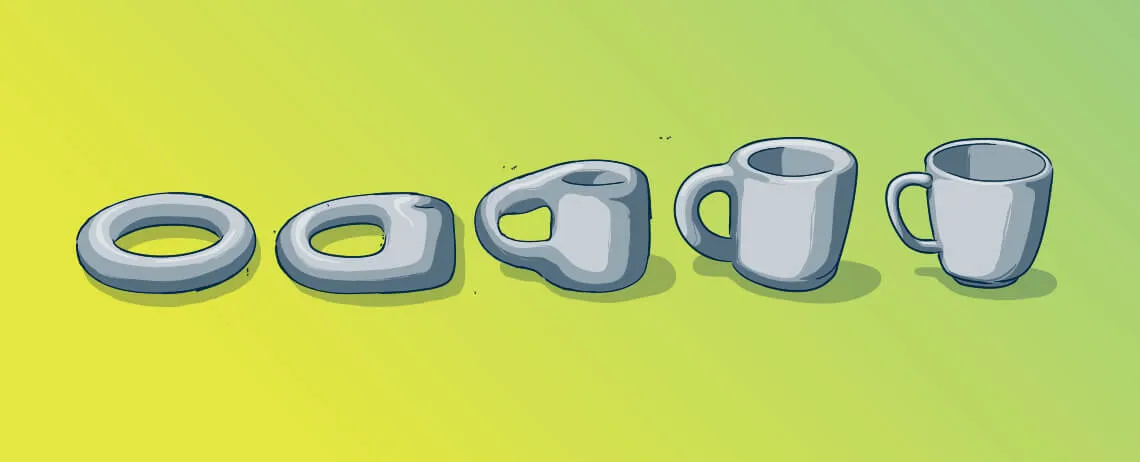
\includegraphics[width=\textwidth]{./img/mbs_02_topology.png}
    \caption[Caption for LOF]{Untrim을 이용한 지오메트리 상태 확인\footnotemark}
    \label{fig:mbs_02_topology}
\end{figure}

\footnotetext{\href{https://www.ctqmat.de/en/showcase/topology}{https://www.ctqmat.de/en/showcase/topology}}
예시를 위해 다음과 같이 3개의 사각형을 그렸습니다. 아래 사각형들은 얼핏 보기에는 같아 보이지만 사실 다릅니다. 그 이유가 무엇인지 설명하도록 하겠습니다(Figure \ref{fig:mbs_03_TopologyRect}).
\begin{figure}[H]
    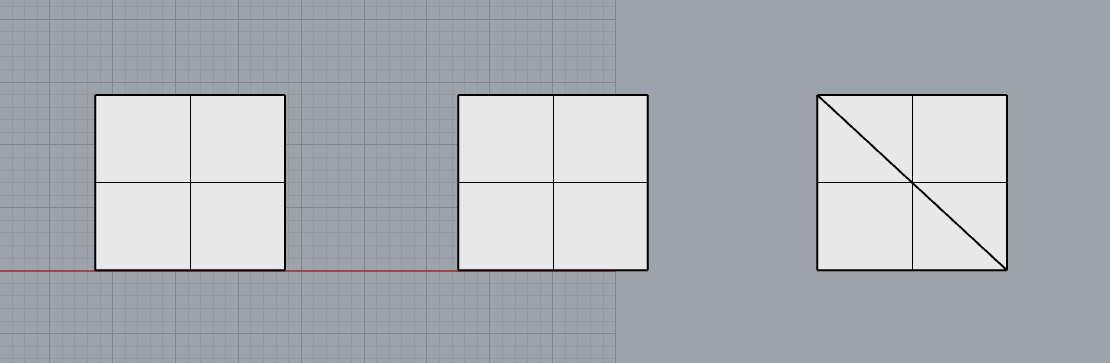
\includegraphics[width=\textwidth]{./img/mbs_03_TopologyRect.png}
    \caption{각각 다른 속성을 가진 3개의 사각형}
    \label{fig:mbs_03_TopologyRect}
\end{figure}

가장 왼쪽에 보이는 사각형은 Rhino에서 사각형을 그린 후, \textit{PlanarSrf} 명령어를 이용해 만든 사각형입니다. 그리고 해당 사각형을 클릭한 후 오른쪽에 위치한 properties 탭을 확인하면, \textit{surface}라고 써있습니다(Figure \ref{fig:mbs_04_SurfRec}). 

\begin{figure}[H]
    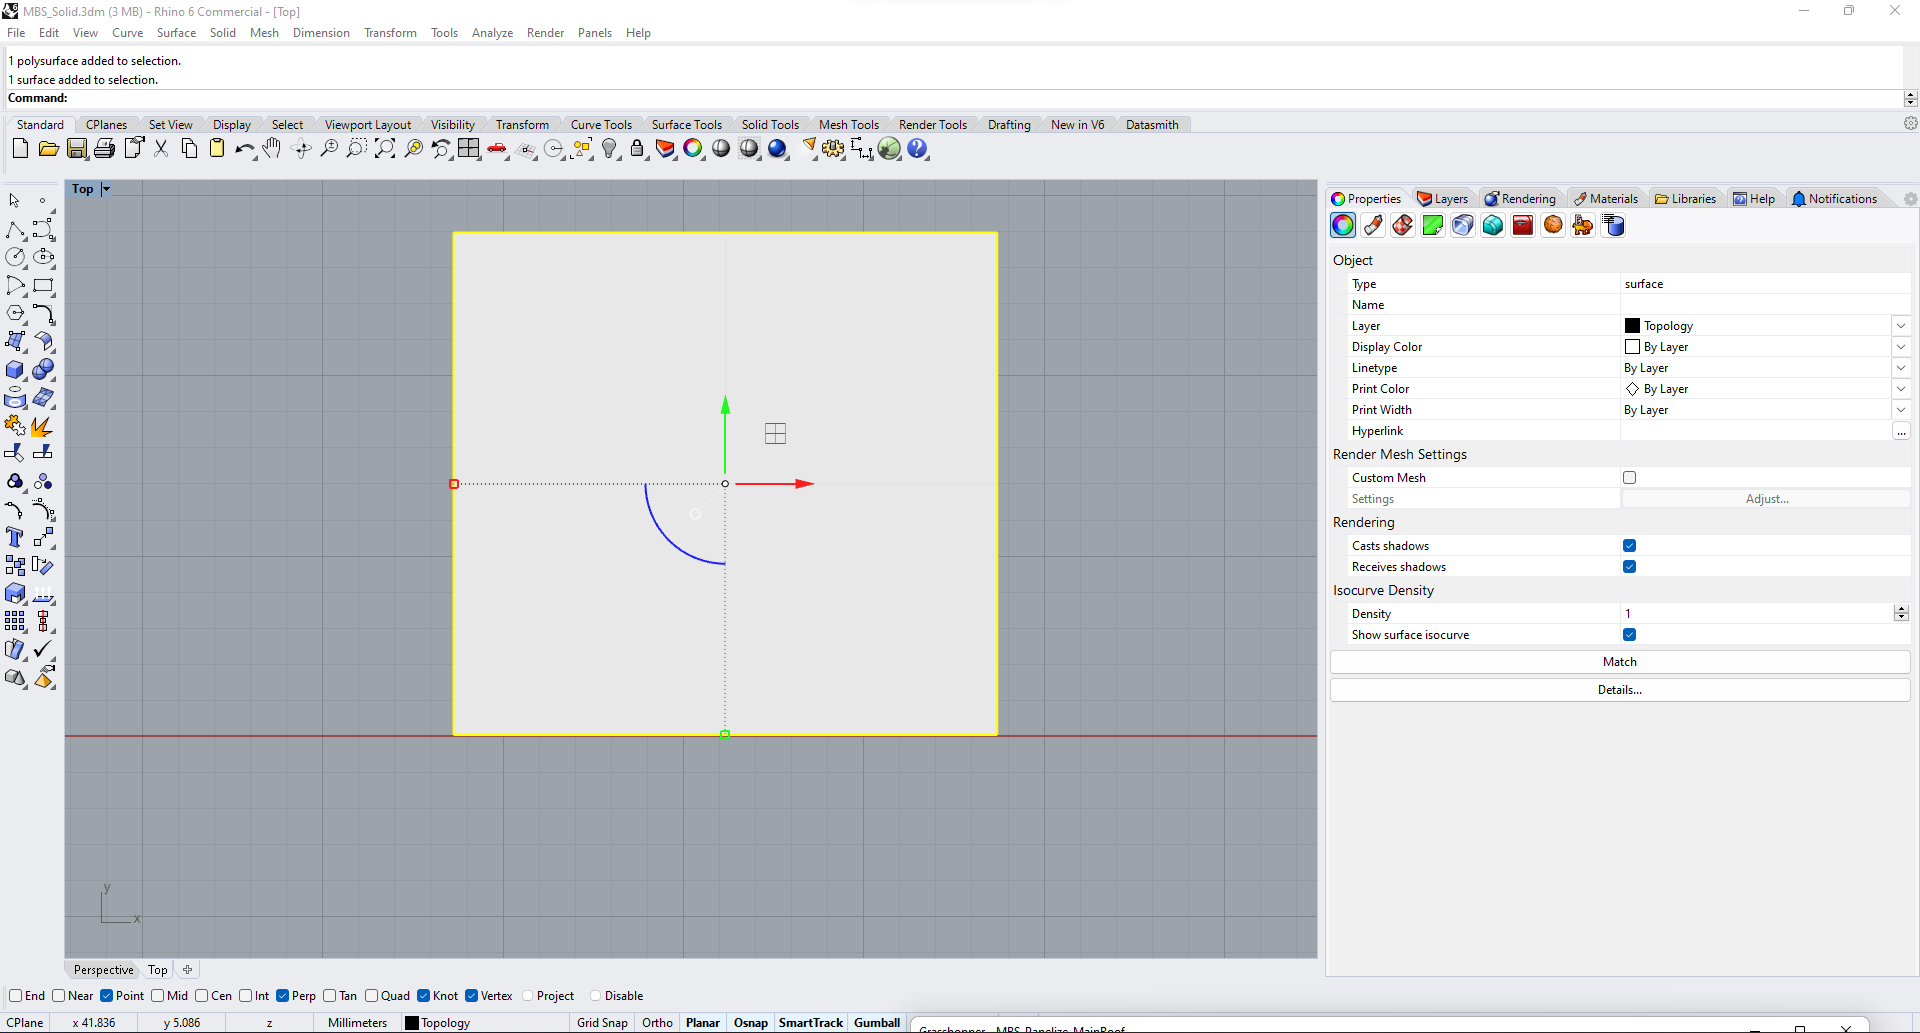
\includegraphics[width=\textwidth]{./img/mbs_04_SurfRec.png}
    \caption{PlanarSrf를 이용해 만든 사각형}
    \label{fig:mbs_04_SurfRec}
\end{figure}
이번에는 중앙에 위치한 사각형을 선택해보겠습니다. 그 후 오른쪽 탭을 확인하면 이번에는 \textit{trimmed surface}라고 나오는 것을 볼 수 있습니다.

\begin{figure}[H]
    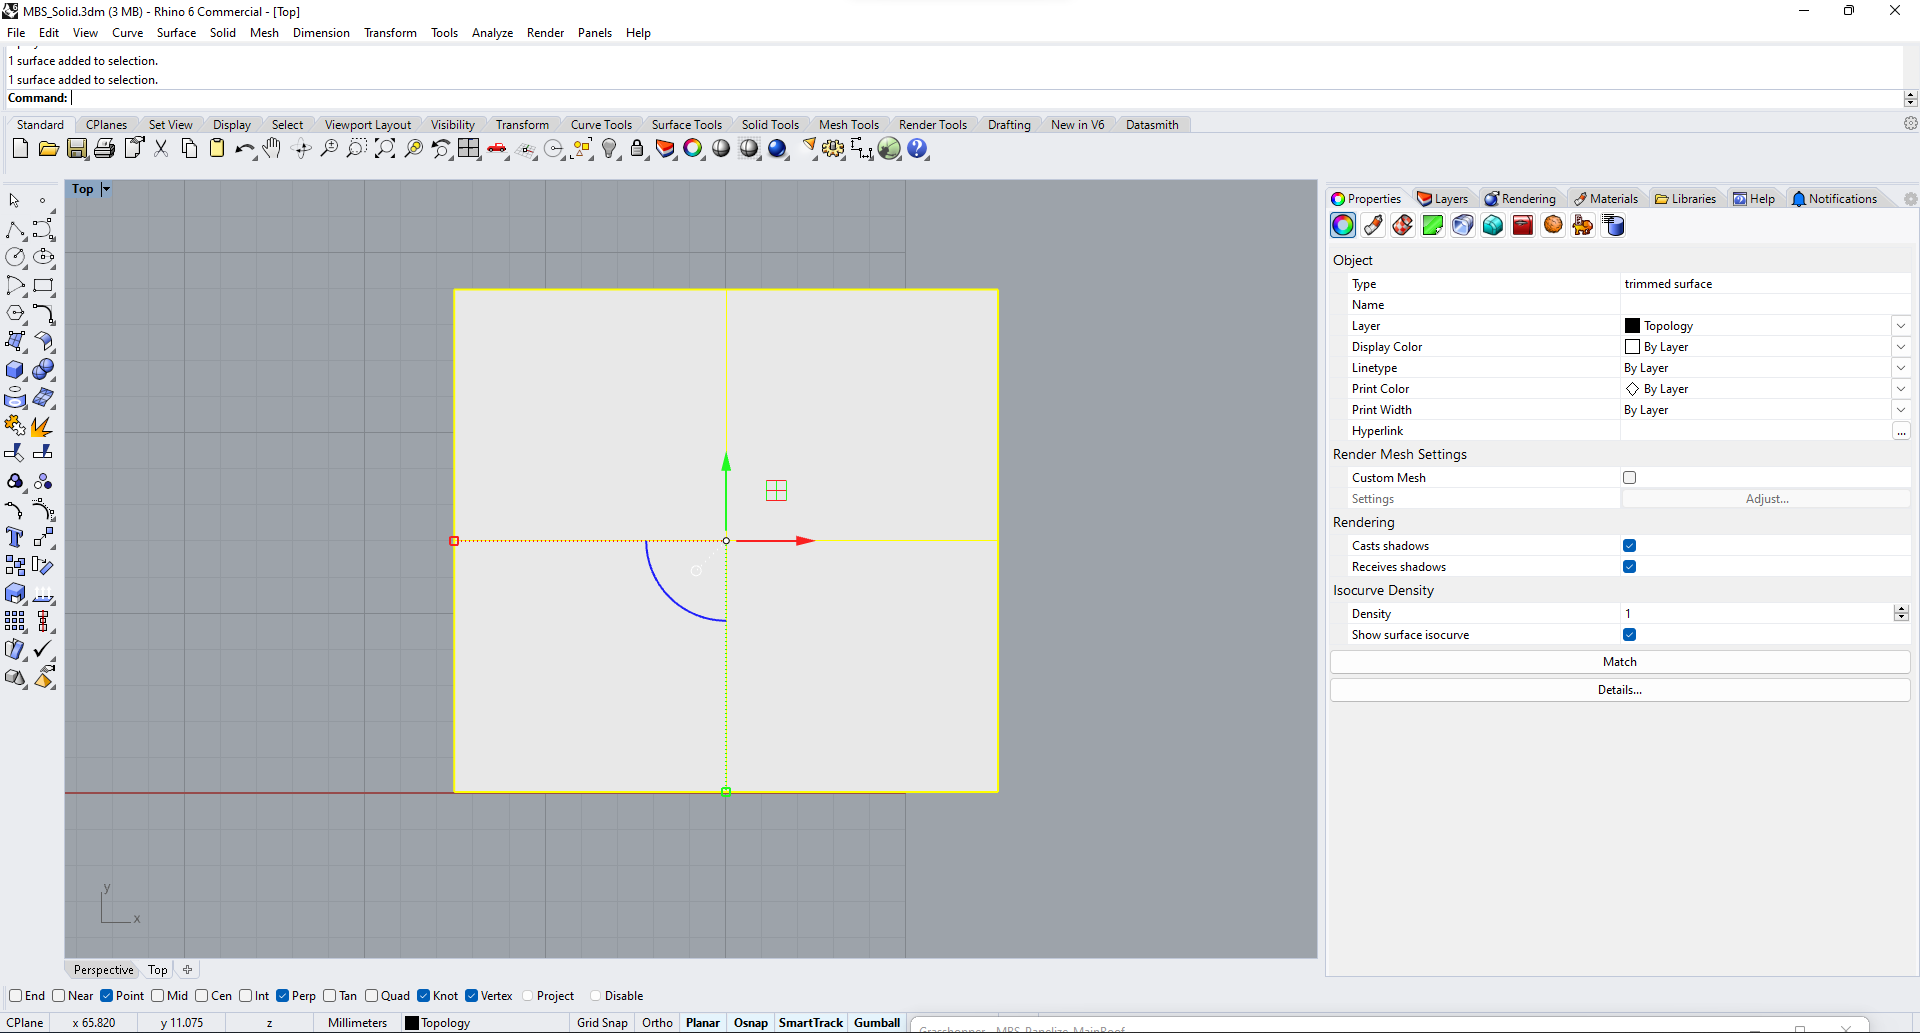
\includegraphics[width=\textwidth]{./img/mbs_05_TrimmedRect.png}
    \caption{사각형을 split해 만든 사각형}
    \label{fig:mbs_05_trimmed}
\end{figure}

마지막으로 가장 오른쪽의 사각형을 선택하고 보면 \textit{open polysurface}라고 나옵니다.

\begin{figure}[H]
    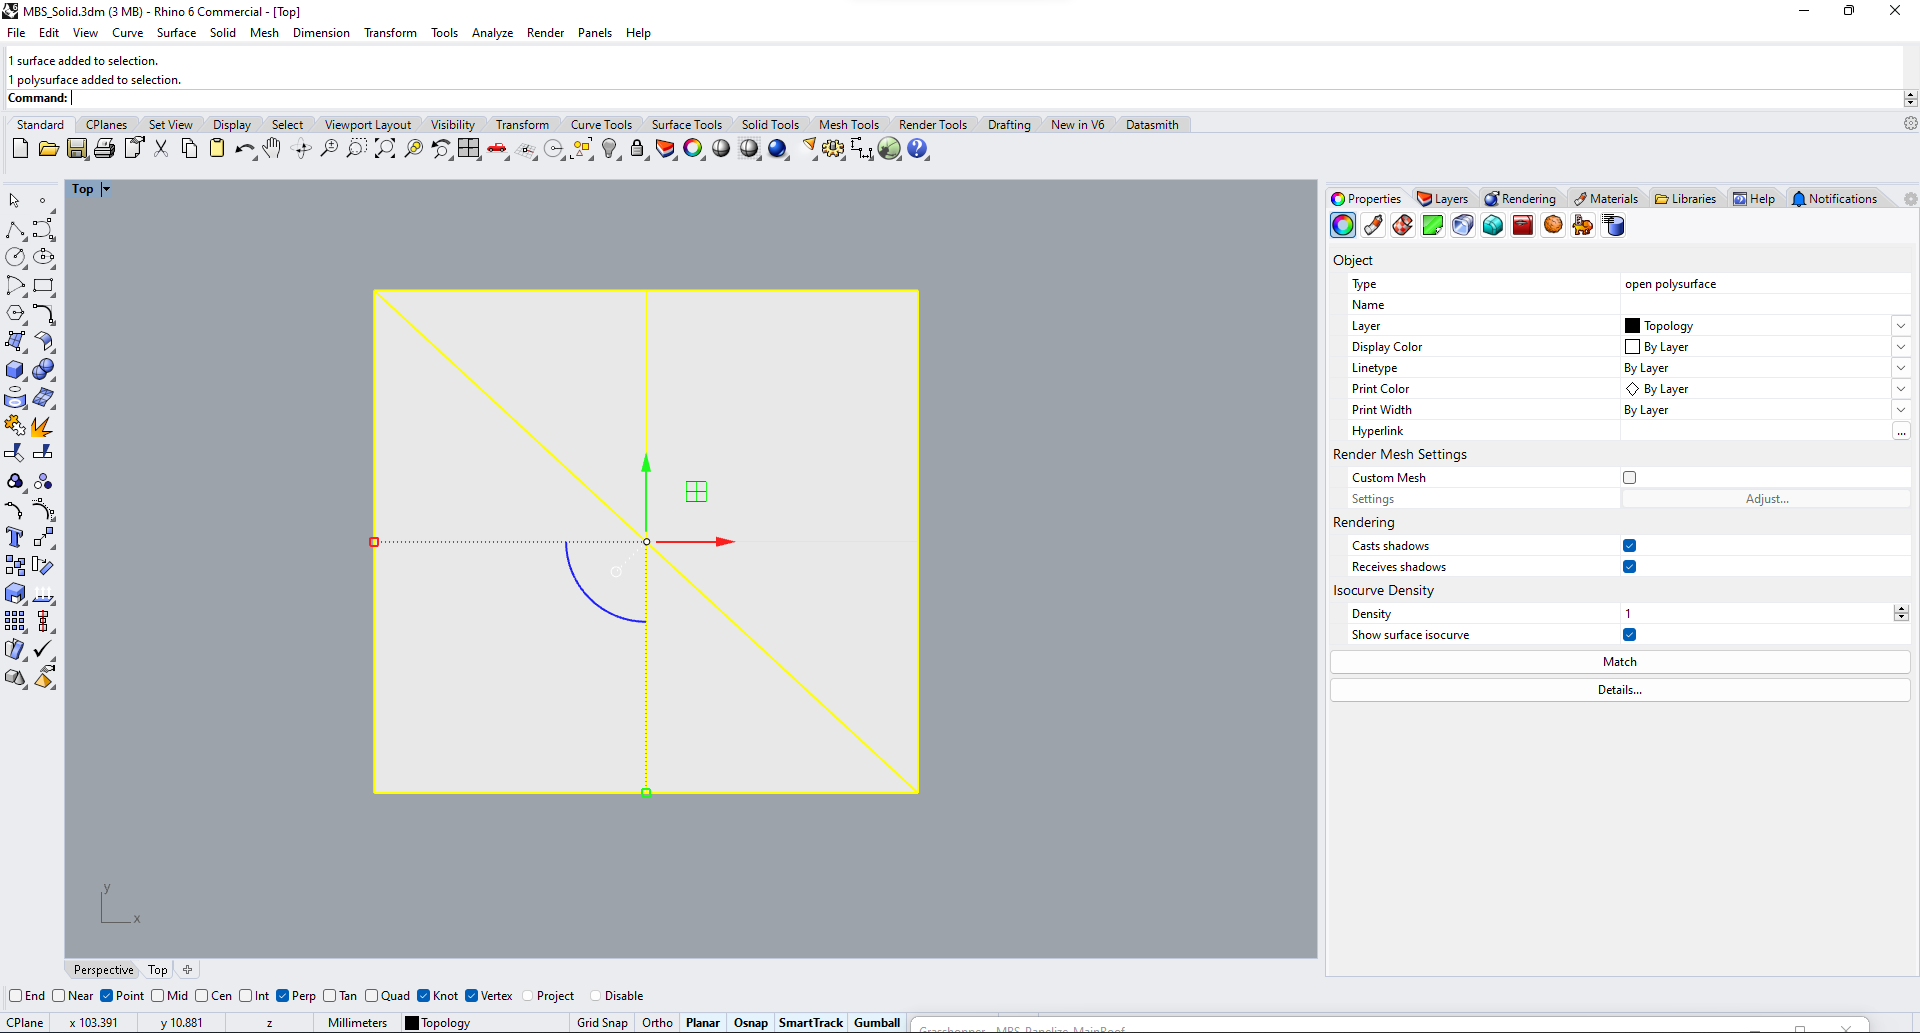
\includegraphics[width=\textwidth]{./img/mbs_06_PolyRec.png}
    \caption{두개의 삼각형을 붙인 사각형}
    \label{fig:mbs_06_polyRec}
\end{figure}
이들이 다른 이유는 당연하게도 지오메트리를 만든 방법이 다르기 때문입니다. 중앙의 사각형은 더 큰 사각형을 만든 후, 현재 보이는 크기 만큼 잘라낸 형태입니다. 그래서 trimmed(잘린) surface라는 설명이 나옵니다.
반대로 \textit{polysurface}는 여러개를 붙인(poly)형태이기 때문에 \textit{polysurface}라고 표시되게 됩니다. 그럼 이 차이가 왜 중요한지를 설명하겠습니다. 결국, 지오메트리의 상태가 다르면 사용해야 하는 명령어도 달라집니다.
그래스호퍼 안에 surface 탭 아래 있는 명령어들은 \textit{surface}를 입력값으로 받는것을 가정하고 만들어진 컴포넌트들 입니다. 따라서 \textit{polysurface}나 \textit{trimmed surface}를 해당 컴포넌트의 입력값으로 사용하면 
오류가 나는 경우가 상당히 많습니다. 제가 모든 경우의 수를 다 해보진 않았지만, 일반적으로 그렇습니다. 

다시 본 강의로 돌아오면 지오메트리를 확인했을때, untrim 명령어를 통해 \textit{trimmed surface}가 아닌것을 확인했습니다. 따라서, 제가 쓰려고 하는 컴포넌트를 쓸 수 있는 조건인 것을 확인했습니다.
\pagebreak

\section{주요 포인트 구하기}
이번 예제의 핵심은 곡률이 있는 원본 지오메트리를 평면삼각형으로 바꾸는 것입니다. 이러한 방법을 도입하기 위해서는 중요한 커브들을 구한후 이들을 나눠 평면 삼각형을 만들때 쓸 포인트들을 구해야 합니다. 이 포인트를 본 글에서는 \textit{주요 포인트}라 하며 주요 포인트를 구할 때 제작 가능한 수치에 맞게 조정하는 과정이 필요한데,
 해당 과정을 중심으로 설명하도록 하겠습니다. 본격적으로 들어가기에 앞서, 몇가지 용어정리를 하도록 하겠습니다. 

모델의 탑뷰(top view)를 기준으로 x 방향을 행방향, y 방향을 열방향이라고 하겠습니다. 그리고 원본 지오메트리의 외곽선을 엣지(edge)라고 하겠습니다(Figure \ref{fig:mbs_07_lang}). 그림 및 설명을 보다가 헷갈리실때는 각 뷰포트의 좌측 하단에 있는 좌표를 보고 판단해주시면 되겠습니다.
\begin{figure}[H]
    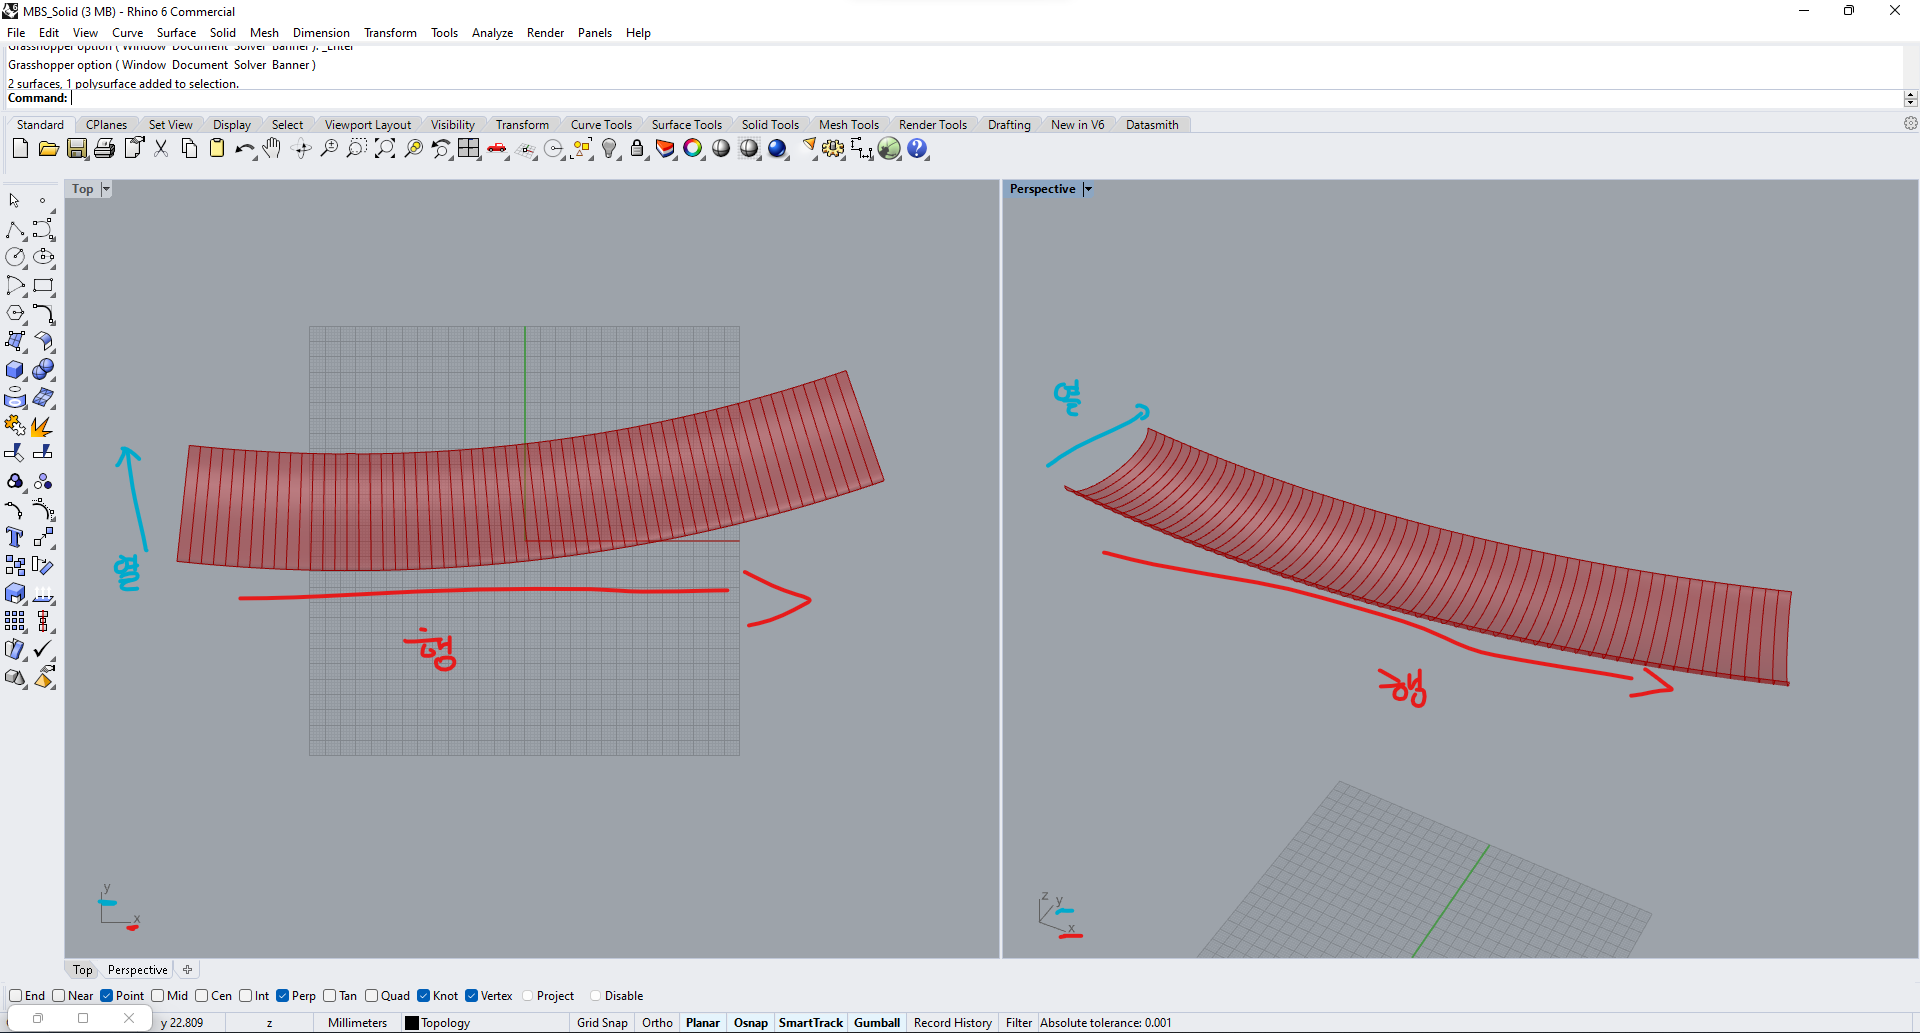
\includegraphics[width=\textwidth]{./img/mbs_07_lang.png}
    \caption{본 글에서 사용하는 커브 방향}
    \label{fig:mbs_07_lang}
\end{figure}
\subsection{가장 긴 엣지 구하기}
앞에서도 계속 언급한바와 같이, 모든 패널이 제작조건에 맞게 생성되야 합니다. 따라서 한 방향에서 가장 긴 엣지 또는 커브를 구한 후, 각 조각이 제작 조건 아래로 떨어지는 숫자로 나누면 제작 조건에 맞는 포인트들을 구할 수 있습니다.
 제작조건을 너비와 높이라 한다면(사실 둘을 교환해도 큰 문제는 없지만) 여기서는 행방향이 최대 제작 가능 너비보다 작도록 설정해보겠습니다. 

이 과정을 수행하기 위해서는 원본 지오메트리에서 가장 긴 엣지를 구하면 됩니다. 한눈에 보기에 행방향에 있는 엣지가 가장 긴것을 볼 수 있습니다. 파라메트릭 모델링을 할때는 아무리 눈으로 보인다해도, 손으로 클릭하는 것이 아닌 논리를 구성해서 작업을 해야합니다.
 왜냐하면 논리를 구성하는 과정인 알고리즘으로 하지 않고 손으로 하는 매뉴얼한 작업을 하게 되면 작업을 자동화 할 수 없습니다. 흔히 Robust한 알고리즘이라는 말을 많이 쓰는데, 패턴이 잘 깨지지 않는 그런 알고리즘을 구성해야 합니다.

\subsubsection{지오메트리를 엣지로 변환}
\subsubsection{Continuity를 이용해 가장 긴 엣지 추출}
\subsection{제작 조건에 맞는 길이로 자르기}
\subsection{UV Curve 기능을 이용해서 엣지에 수직방향 커브 구하기}

\end{document}
